\section{PDCA}
\label{appendiceQualità}
In questo capitolo verrà descritto come è stato applicato il modello \glossario{PDCA} descritto nel \PianoDiQualifica.

\subsection{Revisione dei requisiti}

In questo periodo è stata svolta un attività di \emph{walkthrough} non avendo i dati necessari per effettuare attività di \emph{inspection}, come descritto nel \PianoDiQualifica. Gli errori frequenti rilevati sono visionabili nelle \NormeDiProgetto.

Non è stato possibile eseguire nessun ciclo \glossario{PDCA} in mancanza di misurazioni sui processi, non avendo quindi modo di pianificare processi per la qualità, ma è stato studiato e descritto nel \PianoDiQualifica{} e verrà attuato dalla prossima \glossario{milestone}.

\subsection{Revisione di progettazione}

\subparagraph{PLAN}

Al fine di valutare su quali processi pianificare dei miglioramenti sono state eseguite diverse misurazioni utilizzando le metriche per i processi descritte nel \PianoDiQualifica{}.

I risultati ottenuti sono riportati nella seguente tabella:

\begin{table}[H]
\centering
\begin{tabular}{ | c | c | c | }
\hline
\textbf{Metrica} & \textbf{Valore indice} & \textbf{Esito} \\
\hline
Produttività di documentazione & 199 & Superato \\
\hline
Impegno & 0,71 & Superato \\
\hline
Modifiche & 23 & Non superato \\
\hline
\end{tabular}
\caption{Risultati metriche per i processi, Revisione di progettazione}
\end{table}

Analizzando tali dati si è deciso di pianificare le seguenti attività per il miglioramento della qualità dei processi:

Un numero troppo elevato di modifiche incide pesantemente sulla produttività. È necessario decrementare tale valore al fine di aumentare la produttività e di conseguenza diminuire i costi. Questo primo ciclo \glossario{PDCA} si prefigge dunque l'obiettivo di portare entro un range di accettazione\footnote{Vedi \PianoDiQualifica} il numero di modifiche approvate.

Probabilmente un numero elevato di modifiche è causato dall'inesperienza del gruppo nel primo periodo, e ragionevolmente con l'aumentare delle conoscenze il numero di modifiche andrà calando di conseguenza. 

In ogni caso, si pianifica di:
\begin{itemize}
\item Frammentare maggiormente i task assegnati in sotto-task;
\item Specificare in modo esteso cosa prevede ogni singolo sotto-task, escludendo quindi dubbi che poi porteranno a successive richieste di modifica;
\item Creare la label ``Domanda'' nella sezione \glossario{issue} di \glossario{GitHub}, per permettere la richiesta di delucidazioni sullo svolgimento di \glossario{task} assegnati.
\end{itemize}
  
\subparagraph{CHECK}

Al fine di valutare se le azioni pianificate hanno portato ad un miglioramento dei processi sono state eseguite le necessarie misurazioni.

I risultati ottenuti sono riportati nella seguente tabella:
\begin{table}[H]
\centering
\begin{tabular}{ | c | c | c | }
\hline
\textbf{Metrica} & \textbf{Valore indice} & \textbf{Esito} \\
\hline
Produttività di documentazione & 103 & Superato \\
\hline
Impegno & 2,69 & Superato \\
\hline
Modifiche & 18 & Superato \\
\hline
\end{tabular}
\caption{Risultati metriche per i processi, Revisione di progettazione}
\end{table}

Gli obiettivi posti nello stadio di pianificazione sono stati soddisfatti, si passerà dunque allo stadio di standardizzazione delle soluzioni applicate.


\newpage
\subsection{Revisione di qualifica}
	\subparagraph{PLAN}
	La revisione di qualifica prevede la stesura della Definizione di Prodotto, la manualistica del prodotto e la relativa codifica. La codifica è una una parte corposa e ci aspettiamo una variazione visibile degli indici misurati.

	L'autoformazione svolta fin'ora deve essere testata per verificarne il livello. Per comprendere se il gruppo ha raggiunto le competenze necessarie per affrontare la progettazione di dettaglio e la codifica, e, dove necessario, incrementarle, si pianifica di codificare un prototipo usa e getta assegnando ad ogni componente del gruppo una componente del sistema. Non ci si aspetta che il prodotto derivante da queste attività sia conforme alle attese finali, ma che tutti i membri del gruppo seguano le norme sulla codifica stabilite nelle \NormeDiProgetto{}.
	
	Viene introdotta in questa revisione un'analisi delle issue di \glossario{GitHub} tramite un grafico di \glossario{burndown}. Viene rappresentato il carico di lavoro in relazione al tempo considerando sia il consuntivo sia il backlog, permettendo di confrontare l'andamento reale con quello atteso a fine milestone.
	
	\subparagraph{CHECK}
	La codifica del prototipo ha evidenziato lacune nella formazione sullo stack tecnologico sul quale si appoggia il prodotto. Contemporaneamente, ha contribuito a colmare le stesse lacune e a formare il team in direzione di un processo di codica collaborativo, elemento mancante in molti membri, e coerente con le norme specificate.

	In Figura \ref{fig:burndownRQ} viene riportato il grafico di \glossario{burndown} che si era pianificato di monitorare.
	
	\begin{figure}[H]
		\centering 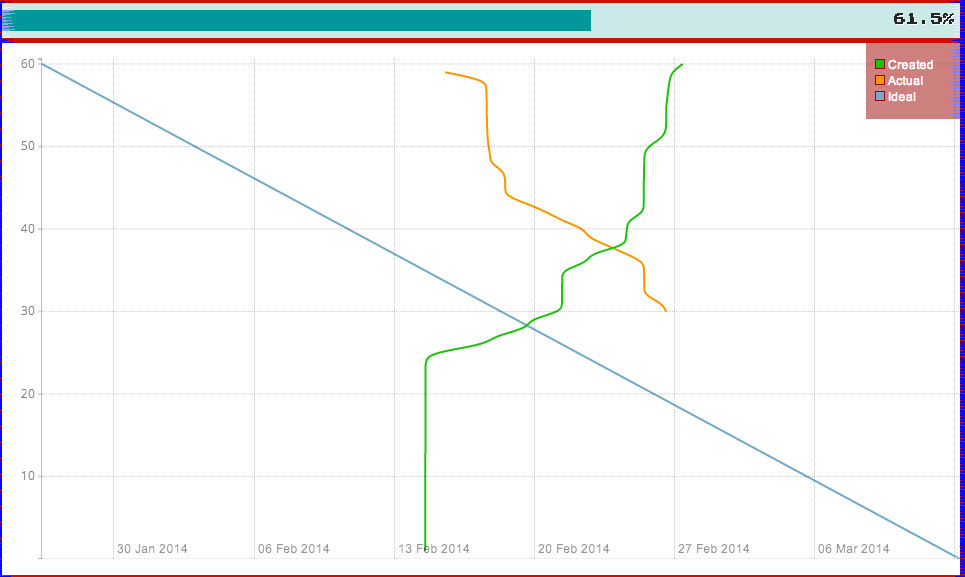
\includegraphics[width=0.8\textwidth]{burndownRQ.png}
		\caption{Burndown RQ}
		\label{fig:burndownRQ}
	\end{figure}
	
	L'esplosione del numero di issue iniziale era atteso poiché le correzioni ricevute dai committenti sono state scomposte in parti atomiche per poterle assegnare ai componenti del gruppo in maniera chiara e tracciabile. Tale grafico si è rivelato utile per comprendere maggiormente l'andamento di sviluppo e accelerare i tempi quando necessario.